
\chapter{Anexo B: Prueba de conocimiento de grafos} \label{AnexoB}
\textbf{Test para verificar aprendizaje de BFS y DFS}

Considere el siguiente grafo:

\begin{figure}[h]
        \centering
    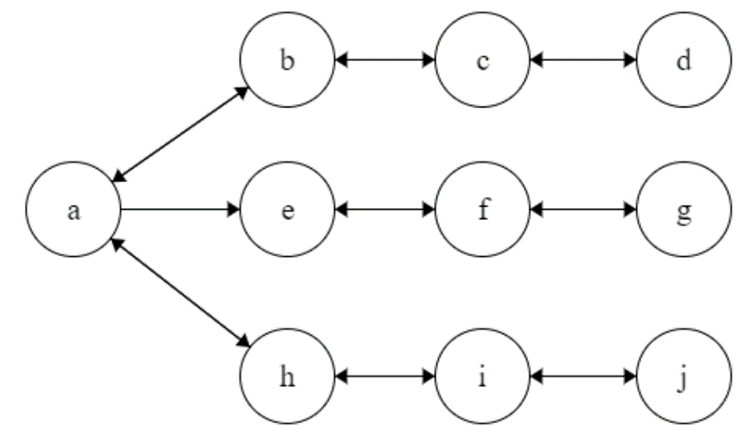
\includegraphics[width=0.6\textwidth]{imagenes/GrafoPrueba.png}
\end{figure}

Muestre el recorrido de un grafo desde el nodo a utilizando distintos los dos algoritmos de búsqueda vistos. \textbf{Agregue una numeración al lado de sus arcos para indicar el orden} en que se explorando.
Por ejemplo, en el siguiente grafo, si se recorre \textbf{a}, \textbf{b} y \textbf{c} partiendo desde \textbf{a, pasando por b y llegando a c}, el resultado esperado es el siguiente:

\begin{figure}[h]
        \centering
        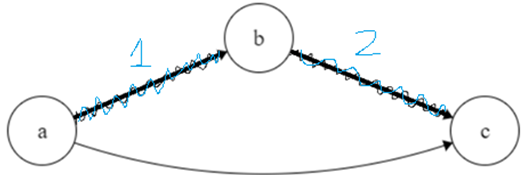
\includegraphics[ width=0.5\textwidth]{imagenes/GrafoPruebaEjemplo.png}
\end{figure}

\newpage 
1.	Aplique el algoritmo \textbf{Búsqueda en Profundidad (DFS / Depth First Search)} para mostrar cómo se recorre un grafo partiendo desde el nodo a.

\begin{figure}[htbp]
        \centering
    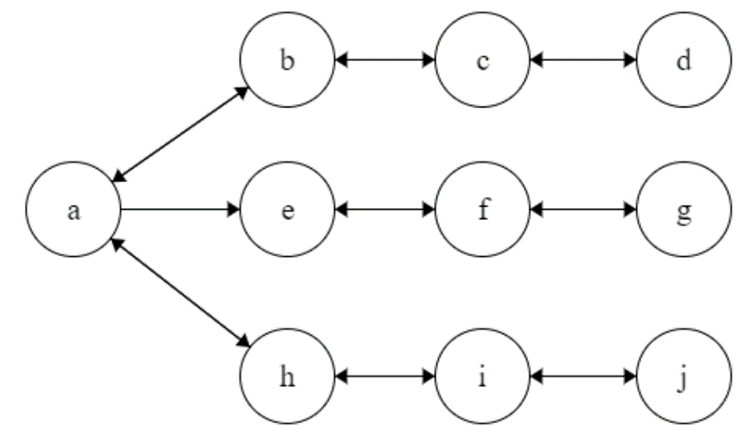
\includegraphics[width=0.7\textwidth]{imagenes/GrafoPrueba.png}
\end{figure}

2.	Repita lo anterior usando el algoritmo de \textbf{Búsqueda en Achura (BFS / Breadth First Search)}

\begin{figure}[htbp]
        \centering
    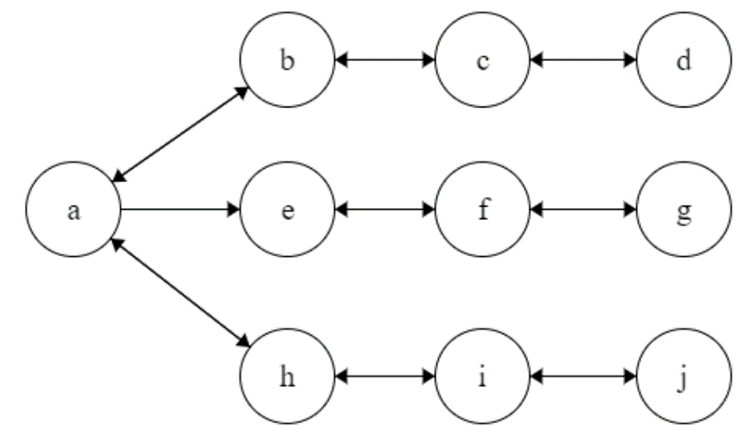
\includegraphics[width=0.7\textwidth]{imagenes/GrafoPrueba.png}
\end{figure}

%\newgeometry{margin=0.1in}
%\begin{figure}[htbp]
    %    \centering
    %    \fbox{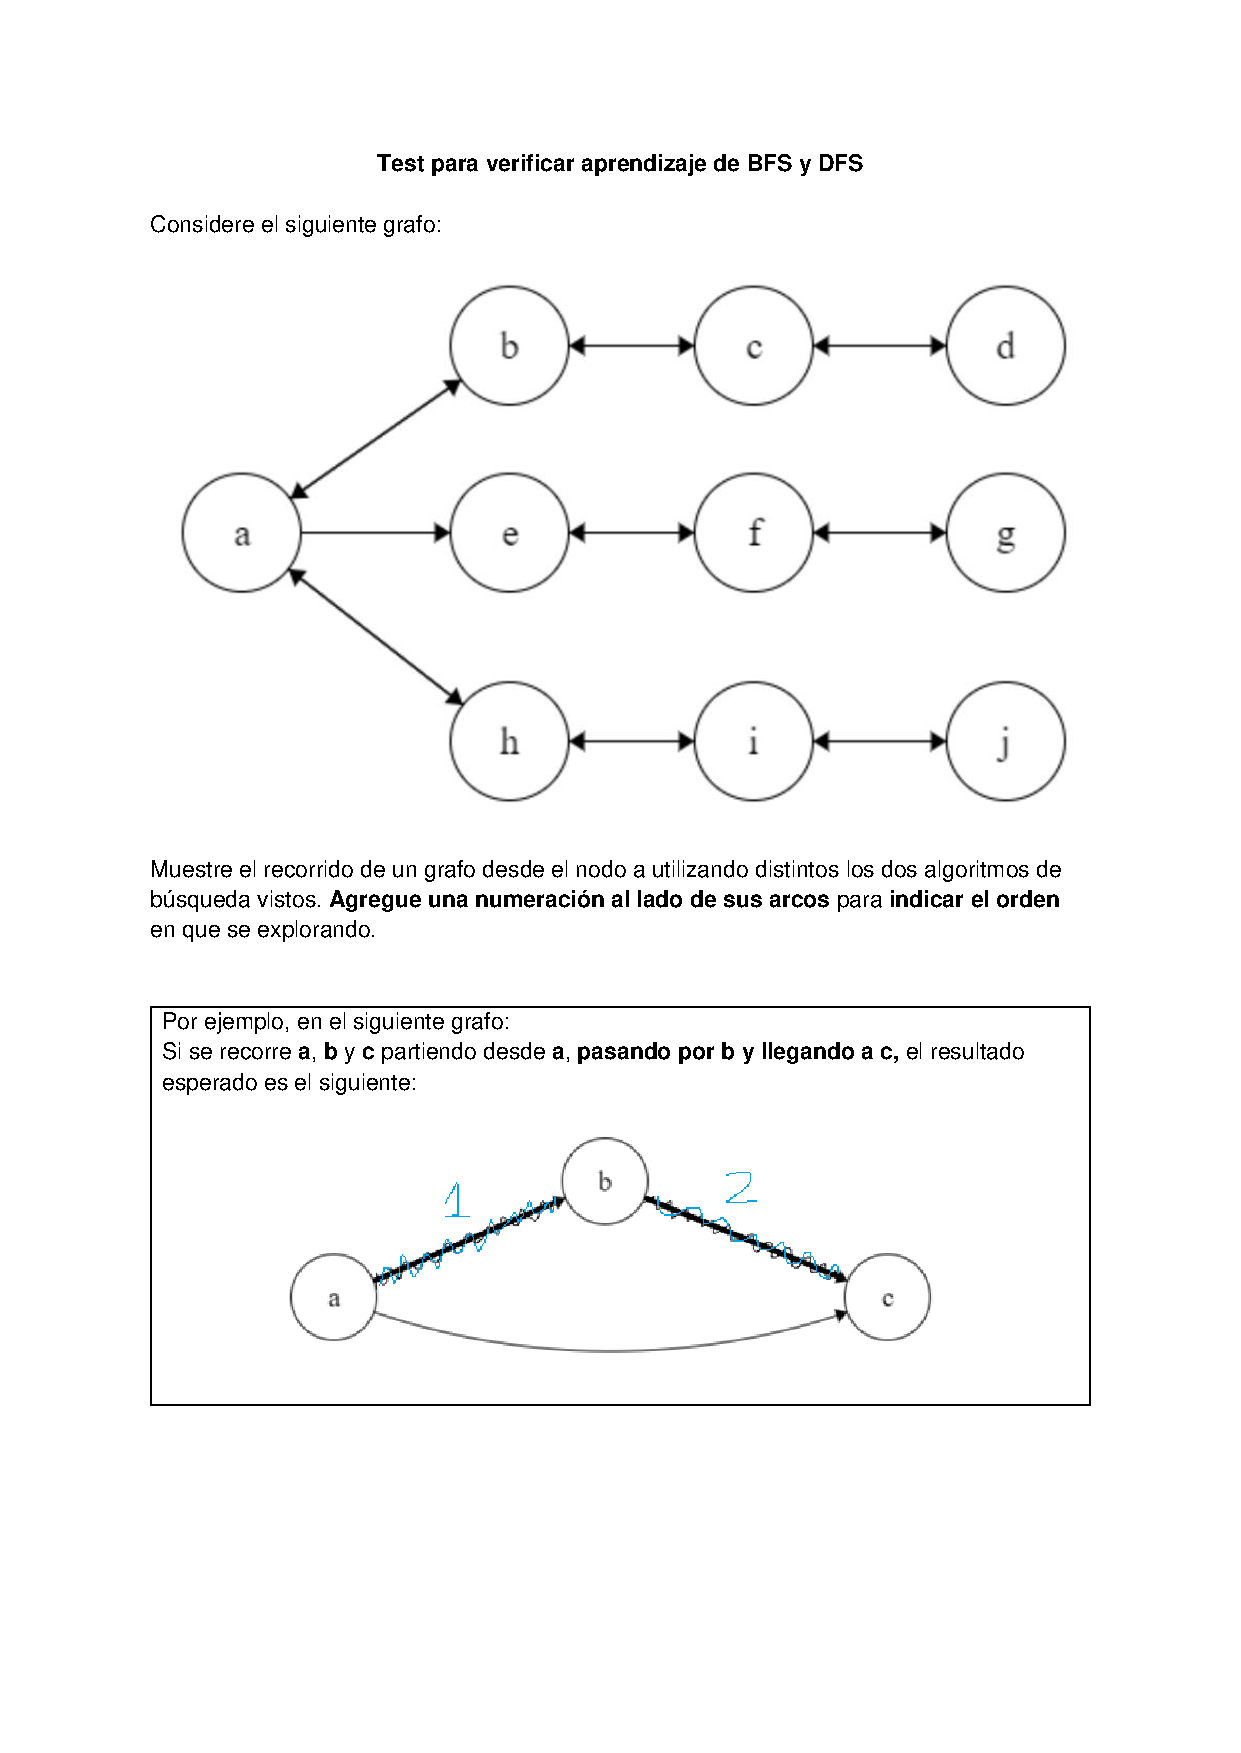
\includegraphics[page=1, width=0.7\textwidth]{imagenes/TestParaVerificarAprendizaje.pdf}}
    %    \caption{Your caption here}
    %    \label{fig:yourlabel}
    %\end{figure}
%\restoregeometry
